I recalled a language arts class in my middle school. This was the source of my opposition to collective responsibility and my earliest philosophical thinking, though I didn't know that ``this was philosophy.'' There were two consecutive texts in my middle school language art textbook: Victor Hugo's \textit{Letter to Captain Butler on the Expedition to China} (\textit{L'Expédition de Chine. Au capitaine Butler}) and Hualing Nieh Engle's \textit{Dear Papa and Mama} (亲爱的爸爸妈妈).

%Previous philosophical thoughts, such as on nationalism, were almost all categorised by me at the time as ``political commentary,'' or political commentary that used scientific (including formal sciences like mathematics) knowledge, like treating the extremist statement ``all Japanese people are guilty'' as a universal proposition and then using Japanese anti-war activists as a counterexample to falsify it. I had never thought that I was thinking about philosophy.

The first text, as its name suggests, is a letter from Hugo to a French captain, criticising the Anglo-French invasion of China. The second text is about a memorial commemoration event of the Nazi massacre in Kragujevac, Yugoslavia. In the event, writers from all over the world discussed ``War and Literature.'' Among them was a West German writer named ``Ming Hebai'' \footnote{``明赫白'' in Chinese. I couldn't find who this person is, what their German name is, or what works they published. It might be a pseudonym created by Hualing to protect them.} who made a statement that I found very confusing:

\begin{quotation}
    The West German writer Ming Hebai slowly stood up. He said gravely, ``\ldots I have a sense of guilt: I feel as if it was I who killed those children. We are simply beasts! All concentration camps must be destroyed! I am very grateful that you allow me to be with you\ldots''
    \par 西德作家明赫白缓缓地站起来,他沉重地说:“……我有犯罪感:感到是我杀害了那些孩子。我们简直就是禽兽!所有集中营都必须粉碎!你们允许我和你们在一起,我非常感激……”
\end{quotation}

I found this passage confusing because of Hugo's article before it, in which Hugo said:

\begin{quotation}
    However, I protest, and I thank you for giving me this opportunity to do so. The crimes of the rulers are not the fault of the ruled; governments may sometimes be robbers, but the people never are.
    \par Mais je proteste, et je vous remercie de m'en donner l'occasion; les crimes de ceux qui mènent ne sont pas la faute de ceux qui sont menés; les gouvernements sont quelquefois des bandits, les peuples jamais.
\end{quotation}

I asked my language arts teacher, why do these two texts contradict each other? If it is as Hugo says, what does the Nazi massacre in Kragujevac have to do with this writer? ``The crimes of the rulers are not the fault of the ruled!'' Hugo did not need to say, ``I feel as if it was I who burned the Old Summer Palace, we are simply beasts.'' That makes no sense.

My teacher said it is normal for different writers to have different views on social issues. You can think for yourself whose view is more reasonable, why, and then share your thoughts with me.

I stood firmly with Hugo: ``The crimes of the rulers are not the fault of the ruled.'' Because the Anglo-French invasion of China was not done by Hugo, and he had no power to stop it, the Kragujevac massacre was not done by Ming Hebai, and he also had no power to stop it. So why should they bear responsibility for things they did not do and could not prevent? Therefore, although Ming Hebai made some seemingly ``profound'' reflections, he essentially still saw himself and the Nazis as ``fellow Germans,'' and his intellectual realm was inferior to Hugo's.

%Then I took the opportunity to criticise some teachers who use collective punishment to maintain classroom discipline. If they couldn't find who was whispering, they would punish all the students in that area. This was not just a classroom opinion, but quickly became a thinking tool for me to understand the world.

At that time, it coincided with the 3/11 earthquake in Japan, and there were some extremist comments on the Chinese internet. I wrote a short story about a Japanese rescue team member who became friends with a Chinese victim of the Wenchuan earthquake when he came to China in 2008. After the 3/11 earthquake, the Chinese person was very worried about their Japanese friend's safety and couldn't contact him. Later, they received an email from the Japanese rescuer's family that he had died in the rescue efforts of the 3/11 earthquake. I found the draft of this story (\cref{fig:notebook}), and I discovered that the story was written from the first-person perspective of a little girl (the victim). Moreover, almost all the fictional stories I wrote at that time were from a girl's first-person perspective. I completely did not notice this issue at the time, and I can find no memory of ever thinking about it.

\begin{figure}[htbp]
    \centering
    \includegraphics[width=0.7\textwidth]{figures/middle_school_notebook}
    \caption{Draft of a short story written by the author in middle school.\label{fig:notebook}}
\end{figure}

This demonstrates that my philosophical views and my gender identity emerged at roughly the same time. They converged after my gender identity became strong enough that I could not ignore, leading me to analyse myself with the intellectual tools that already existed. They may both stem from my childhood experiences. They made me feel that the real world is chaotic and painful, while mathematics, logic, and science is orderly and beautiful. They provided me with a shelter, but this small world is ultimately limited. The external society is still full of irrationality, which drives me to want to completely smash it and rebuild the entire world with mathematics, logic, and science.

This recalls a few small childhood incidents, one of which is that when I was very, very young, I believed that human traffickers did not exist; they were just something my parents made up to scare me. I believed that what I hadn't seen didn't exist. I easily considered it a kind of naive materialism or positivism before I was horrified to realise it was only one step away from subjective idealism.

The statement ``what I haven't seen doesn't exist'' contains two elements:

\begin{enumerate}
    \item ``I'' -- the subject of the judgment.
    \item ``seen'' -- the standard of the judgment.
\end{enumerate}

If I emphasised the ``seen'' and realised that personal ability is limited but still believes in an objectively verifiable physical world, thus extending the subject of ``seen'' from ``I'' to the scientific community or humanity as a whole, and extending ``seen'' to the objective, public ``verifiable,'' one develops towards materialism, positivism, or naturalism. This is the path I took.

If I emphasised the subject ``I,'' and push it to the extreme, the existence of things depends on ``my'' perception, then the entire ``existence'' of things is ``to be perceived.'' Things I cannot perceive do not exist, which leads to subjective idealism.

The thought ``what I haven't seen doesn't exist'' may have been a fork in the road for my personal philosophy. Perhaps the starting points of some completely opposed ideas are much closer than we thought.

Then I realised that my method of analysing the ``non-existence of a complete, ontological gender identity'' is almost identical to \textcite{Hume2007Treatise}'s subjective empiricist argument for the ``non-existence of the self'': I looked inward, saw nothing called ``gender identity,'' only saw many childhood experiences and my reactions to them being artificially grouped together.(\cref{fig:bundle}) The only difference might be that I explained it in a physicalist way as ``reconstructing the training set from the output of a neural network'' and cited scientific research to prove the credibility of memory. \footnote{Hume is considered the precursor of cognitive science, so I was standing on his legacy and reinvented his method.}

\begin{figure}[htbp]
    \centering
    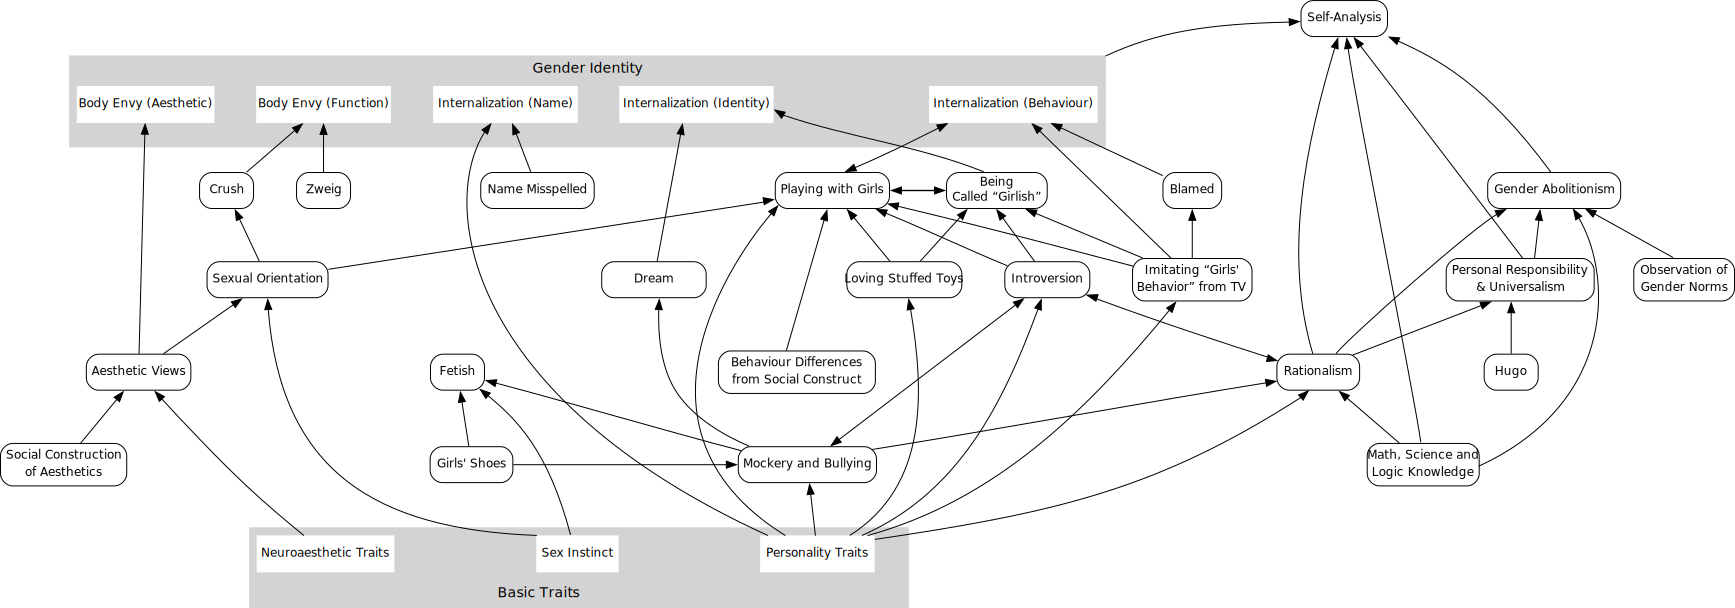
\includegraphics[width=\textwidth]{figures/bundle_of_gender_identity}
    \caption{The author's ``bundle of gender identity,'' like Hume's ``bundle of perceptions.'' Visualised using the Python library graphviz and manually corrected with Inkscape. Due to space and constraint limitations, the neurodermatitis and the events about girls' bathroom are not shown in the diagram.\label{fig:bundle}}
\end{figure}

The second thing is that once, when I was little, I asked my mum, ``Mum, why are you always the one cooking at home? Why doesn't Dad cook?'' My mum said, ``Because Dad is tired of working.'' Then I said, ``You have to work too, aren't you tired?'' My mum was very happy, saying I had grown up and cared for my mum. However, at that time I didn't know what was caring. I just found a logical flaw, which meant that the initial reason was either false, incomplete, or the entire system was built on an unfair double standard. A very similar incident was when I was visiting relatives as a child and questioned the division of kinship terms in our local dialect. I asked my parents why there are more precise terminologies for paternal relatives than for maternal relatives, and they responded with ``it's tradition, don't ask stupid questions.''

%Many years later, I learned that this was precisely the ``categorical imperative'' proposed by Kant centuries ago: only follow the maxim that could become a universal law. The young me discovered that my mum's reason, ``if you're tired from work, you don't have to cook,'' could not become a universal law, otherwise nobody would cook, and we will be starved to death, no rational person would will such a world. This meant that the initial reason was either false, incomplete, or the entire system was built on an unfair double standard. \footnote{I support Kant's ethics but not the transcendental idealism. I had tried to abandon Kant's metaphysics and rebuild the normative part of his ethics in a physicalism worldview, which seemed very difficult, and I ultimately did not complete it. }

%The true, unstated maxim was likely not about tiredness at all, but about socially prescribed gender roles. The actual operating principle might have been something like: ``The woman in the household is responsible for cooking, regardless of her tiredness.'' When subjected to the categorical imperative, this maxim also fails. A rational being cannot will a universal law that assigns duties based on arbitrary characteristics like gender rather than on a fair, impartial, and rational distribution of labor. Such a law would treat certain rational agents merely as a means to get food, which violates Kant's second formulation of the categorical imperative, the Formula of Humanity.

% my mother's brothers and male cousins were all ``jiù'' (舅), and her sisters and female cousins were all ``yí'' (姨). My father's sisters and female cousins were all ``gū'' (姑). In contrast, my father's brothers and male cousins were divided into three categories: elder brother and male cousins were ``dàyé'' (大爷), younger brother and male paternal cousins were ``dàda'' (大大), and younger maternal male cousins were ``biǎoshū'' (表叔)

These memories led me to examine a more fundamental question: where does my obsessive need for systematicity and logical consistency come from? Is it merely an acquired academic habit, or does it have deeper roots? In the process of exploring my ``gender identity,'' I unexpectedly found a possible answer. Research on atypical gender experiences is sometimes associated with autism spectrum disorder (ASD). Initially, I did not associate this with myself, but these cognitive traits, like analytical understanding, systematic thinking, and problems in understanding social norms, highly resemble my experience.

I started to consider the possibility that I might have ASD or a subclinical Broader Autism Phenotype (BAP). As a self-test, I scored 36 in the Cambridge Autism-Spectrum Quotient \parencite{BaronCohen2001Autism}. Although this result cannot be used as a diagnosis, it can be used as a heuristic explanatory framework for understanding myself. Of course, my case might not be typical: autistic individuals usually have a strong interest in a specific area, whereas my interest is almost in the entire world.

It should be noted that this does not constitute a biological determinism, and does not overturn my previous hypotheses about the origin of my preference for science and logic. The ``special interests'' of autistic individuals are remarkably diverse, and everyone's ``special interest'' is also formed through interaction with society. An autistic child cannot innately know what a dinosaur or a train is. The main reason for my ``interest'' is still likely due to a deep hatred of the illogical real world. Without this experience, my ``special interest'' might also be a specific field. My experience of order in science and logic and the subsequent willingness to rebuild the entire world are not an inevitable result of autism, but my own agential choice. The biological determinist assumption that my love for reason and science was directly originated from the autistic traits is absurd because it is somewhat implying that all scientists and philosophers are autists.

This discovery also provided new evidence for my view that ``neutral innate neural traits are assigned gender labels by society and culture.'' In the research I read on ASD (including previous Asperger's syndrome), there were two papers on FtM or FtX individuals who said they felt not like females or were more like males since childhood. One paper's author followed Dr Hans Asperger's original view from his 1944 description, that ``the autistic personality is an extreme variant of male intelligence,'' and considered the neurological traits of autism to be a so-called ``male brain'' \parencite{Kourti2019Dont, Kraemer2005Comorbidity}.

However, my own situation is more complex. As a child, I disliked socialising and preferred to read and think alone. I was told by elders that I was like a little girl and was bullied by classmates. This is the exact opposite of Dr Hans Asperger's classic explanation. Yet, as an adult, I am considered ``very masculine'' because of my logical thinking style, and some TERFs have claimed that ``your way of thinking is male, you don't understand our female experience at all.'' The biological basis is neutral. How it is interpreted by society and culture, how this interpretation acts on an individual, and what kind of self-identity the individual ultimately forms are largely arbitrary. Without society and culture, it is just a neurological trait that has nothing to do with ``gender.''

How it is interpreted and what ``gender'' it is assigned depends entirely on the external sociocultural framework, the observer's position, and even an instrumental purpose in a specific context -- whether it is describing a quiet child with a ``good'' faith or attacking a debate opponent with a bad faith. The interpretation is not based on any objective, consistent standard, but serves the interpreter's own agenda.